\documentclass[journal]{IEEEtran}
\usepackage{algorithmic}
\usepackage{array}
\usepackage{url,amsfonts,amsmath,amssymb,amsthm,color,enumerate,tikz,hyperref}
\usepackage{algorithm,bbm}
% \usepackage{indentfirst}
\usepackage{stackrel}
\usepackage{listings}
\usepackage{subfigure}
\usepackage{subfloat}
\usepackage[justification=centering]{caption}
\usepackage{booktabs} % for three-line table
% \usepackage{subfig}
\usepackage{graphicx}
\ifCLASSINFOpdf
\else
\fi
\hyphenation{op-tical net-works semi-conduc-tor}


\begin{document}
\title{Name Trend Prediction\\Data Project Report for EECS 564}

\author{Yu Wang% <-this % stops a space
% \thanks{}% <-this % stops a space
}

% The paper headers
% \markboth{}%
% {}
\maketitle

\begin{abstract}
Names given by parents are more than just an identification, but also reflect the fashion of that time. 
% According to the dataset, 30274 distinct names have been used. 
As expected, new names keep springing out, some names are long lasting and some names may be more and more desolate in the future. This project will apply a Matched-Filter-based slope filter to detect the trend of the popularity. For booming period, an Epidemic Model for Name will be implemented to explain the data. After that, a model for the growth of popularity of new names will be proposed based on the result from the previous two steps. 
\end{abstract}

\begin{IEEEkeywords}
Names for Babies, Popularity, Epidemic Model, Prediction
\end{IEEEkeywords}

\IEEEpeerreviewmaketitle

% Abstract / Introduction (sub: Data) / Problem Formulation and Models / Methods / Results

% In the Introduction section, have a subsection that describes your data. In the Problem Formulation and Models section, describe the problem you are trying to solve as precisely as possible. Then describe the model you are using for your estimation/filter/detection etc. In the Methods section, describe your approach and those that you compare with. In Results, describe any experimental results on your data (and theoretical results if you have any).
\footnote{Code can be download through \url{https://github.com/qizhu8/Name_Trend_Prediction}}

\section{Introduction} % (fold)
\label{sec:introduction}
Undoubtedly, everyone has a name. Parents prefer to choose names they heard about before like James and Mary, rather than random generated name like Akdbsts. In this project, we believe the spreading of a name can be described with the same model for virus, which is often called Epidemic Model\cite{Epidemic_Model_SIR}. Intuitively, when one couple of pioneer parents give a lovely name for their baby, their neighbors, colleagues, relatives and everyone who can have access to this piece of information will help them spread this new name. If some people give this name to their babies afterwards, a new round of spreading begins. This procedure is similar to the one that one person in the office catches cold, and several days later, many other people begins to cough. Epidemic Model is reasonable to fit this procedure. In this project, a modified model called Epidemic Model for Name(EMN) will be proposed.

However, EMN will show its power only for ``spreading procedure''. According to the dataset, most names are not undergoing purely spreading or fading procedure, but the combination of both or even more complex ones. So, the first step is to tag the trend with ``increasing'' and ``decreasing'', and focus on ``increasing'' part. The most common and naive idea to split the whole trend from 1910 to 2015 for this problem is by examining  the ``slope'' of the curve. However, because of the existence of noise, ``slope method'' is not that robust. In this project, a Matched-Filter-based slope detector will be implemented. Matched-Filter\cite{gubner2006probability} is the optimal solution for signal detection when the noise is AWGN(Additive White Gaussian Noise). With the help of the new detector, we can split the trend of each name more properly.

The power of Epidemic model is not limited only to fit the trend of names, but also predict the future for them. In the end, this report will also predict the future states from some names, and will propose a most likely model for the growth of a newly come up name. 
\subsection{Dataset} % (fold)
\label{ssub:dataset}
The dataset is given by the Social Security Administration\cite{Social_Security_Administration}. The file can be downloaded through the link \cite{namesbystate}. This dataset stores names' usage information for each 50 states from 1910 to 2015. To safeguard privacy, names used by less than five people in one state one certain year will not show up in the file. 
Each record contains state, gender, year, name and occurrence . The following record is an example of one instance in file ``AK.TXT''
\[
	\underbrace{AK}_{State},~~\underbrace{F}_{Gender},~~\underbrace{1910}_{Year},~~\underbrace{Mary}_{Name},~~\underbrace{14}_{\#~of~users}
\]
The above record means that, in 1910 Alaska, 14 female babies were given name ``Mary''. 
% subsection dataset (end)

% section introduction (end)

\section{Problem Formulation \& Models} % (fold)
\label{sec:problem_formulation_&_models}
By the description of introduction in section \ref{sec:introduction}, three targets will be reached one by one in this project.

\subsection{Trend Detection} % (fold)
\label{sub:trend_detection}
The goal for Trend Detection step is to tell whether this point on the curve is in increasing or decreasing period. We should tell whether the slope for this point is greater or less than 0.

Denote the function of the curve for the name to be $y = f(t)$. For time $t'$, we need to tell whether $k' = \frac{d f(t)}{d t}|_{t = t'} \lessgtr 0$. 

In reality, the above method is prone to noise. In other word, the slope $k'$ may fluctuate round $0$ too often. 
\begin{figure}[ht]
\centering
\subfigure[Mary]{
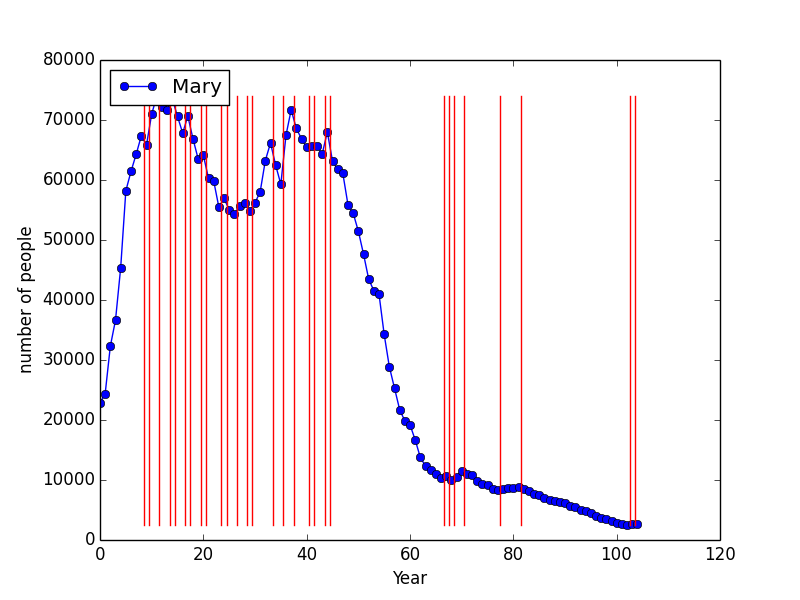
\includegraphics[width = 1.5in]{figure/0Mary_slope_detector.png}
\label{fig:Mary_slope_detector}
}
\quad
\subfigure[Ashley]{
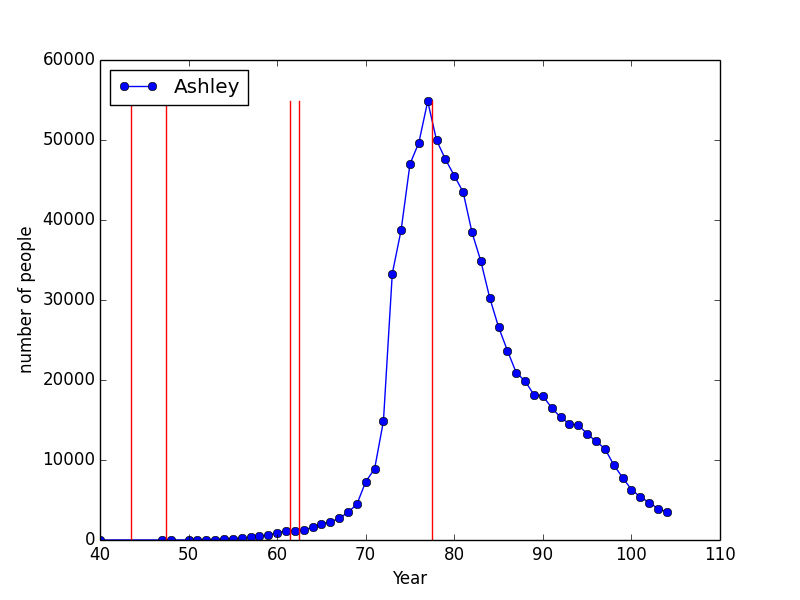
\includegraphics[width = 1.5in]{figure/17Ashley_slope_detector.png}
\label{fig:Ashley_slope_detector}
}
\caption{Performance for Common Slope Detector}
\label{fig:Performance for Slope Detector}
\end{figure}

Fig.\ref{fig:Mary_slope_detector} and \ref{fig:Ashley_slope_detector} are two typical examples of the situation described above. Red line stands on places where the monotonicity flips. For the name ``Ashley'', we know that there is roughly one peak, and the trend is firstly going up and then going down, that simple. Because of the existence of noise, the incline part is not that smooth. As a result, many ``False'' detections are made. So do the curve for ``Mary''.

In order to make the slope detector more robust to noise, we would like to take into more points to make the decision. Then we think of the idea for Matched-Filter\cite{gubner2006probability}.

In this model, we assume the noise is zero mean Additive White Gaussian Noise (AWGN), with power $\sigma^2$. Also, $k \geq 0$ and $k < 0$ are equally likely.
Suppose the true signal $x(t)$ is a linear function with constant slope $k$. Then the expression of the curve would be:
\begin{align}
	y(t) = \underbrace{k \cdot t}_{x(t)} + b + n ~~~ n \sim \mathcal{N}(0, \sigma^2), t \in \{1, 2, \cdots, m\}
\end{align}

Our target is to tell whether $k$ is greater or less than $0$. Then we think about the following model for detection.
\begin{figure}
	\centering
	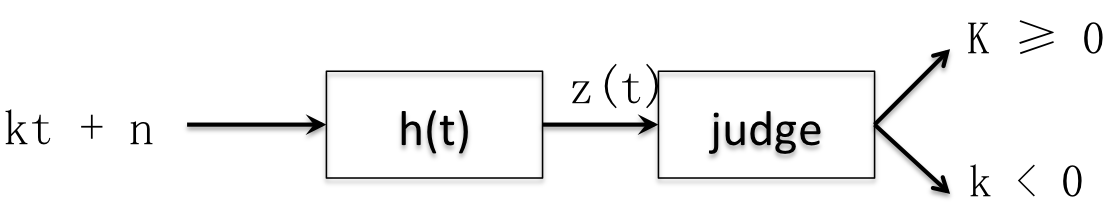
\includegraphics[width = 3.1in]{figure/MF_detector_diagram.png}
	\caption{Diagram for Matched-Filter-based Slope Detector}
	\label{Diagram for Matched-Filter-based Slope Detector}
\end{figure}
The hypothesis test for this problem is:
\begin{align*}
	\begin{cases}
		\mathcal{H}_0: k \geq 0\\
		\mathcal{H}_1: k < 0
	\end{cases}\\
	p(\mathcal{H}_0) = p(\mathcal{H}_1) = 1/2
\end{align*}

Denote $h(t)$ to be the patten we will use, then $t_0$ is the length of patten we are interested in. If $t_0 = 3$, it means we will make our decision based only on the point itself and previous, afterward one point.
For $\mathcal{H}_0$, $k \geq 0$, then $z(t)$ is:
\begin{align}
	z(t | \mathcal{H}_0) &= \sum_{t = 0} ^ {t_0 - 1} h(t)\big((t_0 - t) |k| + b n(t)\big)\\
		 &= |k|\sum_{t = 0} ^ {t_0 - 1} h(t)(t_0 - t) + \sum_{t = 0} ^ {t_0 - 1} h(t) (b + n(t)) \label{eq:H0 output of h(t)}
\end{align}

For $\mathcal{H}_1$, $k < 0$, then $z(t)$ is:
\begin{align}
	z(t | \mathcal{H}_1) &= \sum_{t = 0} ^ {t_0 - 1} h(t)\big(-(t_0 - t) |k| + b + n(t)\big)\\
		 &= -|k|\sum_{t = 0} ^ {t_0 - 1} h(t)(t_0 - t) + \sum_{t = 0} ^ {t_0 - 1} h(t) (b + n(t))\label{eq:H1 output of h(t)}
\end{align}

$z(t | \mathcal{H}_0)$ and $z(t | \mathcal{H}_1)$ are not the likelihood, but the power of output at time $t_0$. For the output, the one with larger Signal Noise Ratio(SNR) will win. So we get to the following expression:
\begin{align}
	z(t | \mathcal{H}_0) \mathop{\lessgtr}\limits_{\mathcal{H}_0}^{\mathcal{H}_1} z(t | \mathcal{H}_1)
\end{align}

According to \ref{eq:H0 output of h(t)} and \ref{eq:H1 output of h(t)}, we know that the only difference between them is the sign for $k$. We can choose $h(t)$ such that 
\begin{align}
		& z(t | \mathcal{H}_0) \mathop{\lessgtr}\limits_{\mathcal{H}_0}^{\mathcal{H}_1} z(t | \mathcal{H}_1) \\
	\Rightarrow &
		|k|\sum_{t = 0} ^ {t_0 - 1} h(t)(t_0 - t) + \sum_{t = 0} ^ {t_0 - 1} h(t) n(t) \nonumber\\
	& \mathop{\lessgtr}\limits_{\mathcal{H}_0}^{\mathcal{H}_1} -|k|\sum_{t = 0} ^ {t_0 - 1} h(t)(t_0 - t) + \sum_{t = 0} ^ {t_0 - 1} h(t) n(t) \\
	\Rightarrow &
		\sum_{t = 0} ^ {t_0 - 1} h(t)(t_0 - t) \mathop{\lessgtr}\limits_{\mathcal{H}_0}^{\mathcal{H}_1} -\sum_{t = 0} ^ {t_0 - 1} h(t)(t_0 - t) \\
	\Rightarrow &
		\sum_{t = 0} ^ {t_0 - 1} h(t)(t_0 - t) \mathop{\lessgtr}\limits_{\mathcal{H}_0}^{\mathcal{H}_1} 0
	\label{eq:simplified expression for hypo test}
\end{align}

From expression \ref{eq:simplified expression for hypo test}, we know that any $h(t)$ satisfies the inequality will work. So in this project, we choose $h(t) = t - t_0/2$. So, if choose $t_0 = 9$, then $h(t)$ is a sequence like $\{4.5, 3.5, 2.5, 1.5, 0.5, -0.5, -1.5, -2.5, -3.5, -4.5\}$.

So to tell whether $f(t')$ is in increasing mode, we will apply convolution to get the value after applying the patten.
\begin{figure}[ht]
\centering
\subfigure[Mary]{
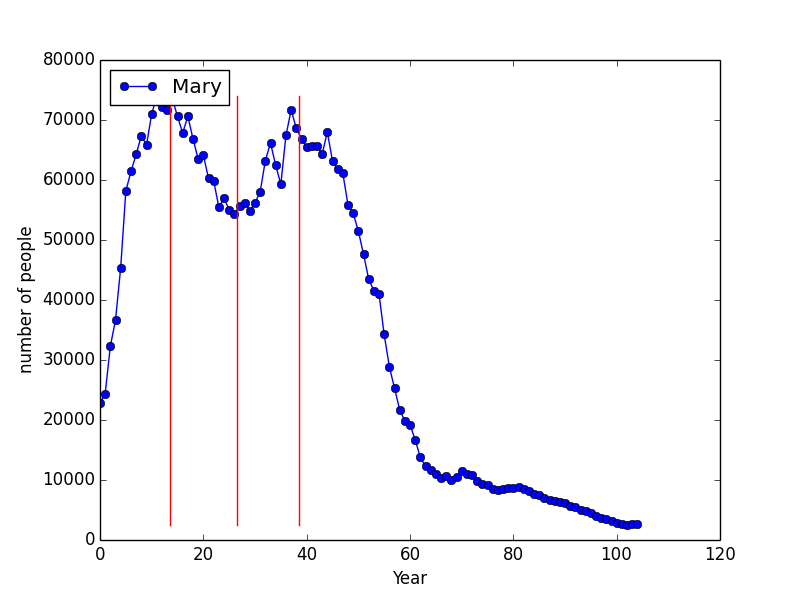
\includegraphics[width = 1.55in]{figure/0Mary_MF_detector.png}
\label{fig:Mary_MF_detector}
}
\quad
\subfigure[Ashley]{
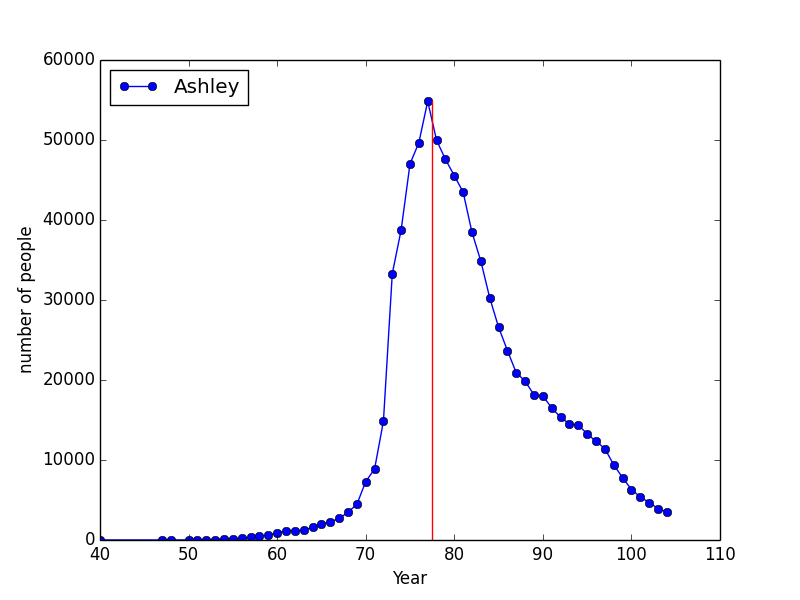
\includegraphics[width = 1.55in]{figure/17Ashley_MF_detector.png}
\label{fig:Ashley_MF_detector}
}
\caption{Performance for Matched-Filter-based Slope Detector}
\label{fig:Performance for Matched-Filter-based Slope Detector}
\end{figure}

Fig.\ref{fig:Performance for Matched-Filter-based Slope Detector} shows the result for Matched-Filter-based Slope Detector for name ``Mary'' and ``Ashley''. Obviously, the performance is much better then the naive method. 

% subsection trend_detection (end)

\subsection{Epidemic Model for Name} % (fold)
\label{sub:Epidemic Model for Name}
Epidemic Model for Name shares the same idea from SIR model \cite{Epidemic_Model_SIR} in 1994. We think the spread of a new name is similar to the epidemic of virus. 
After the Trend Detection \ref{sub:trend_detection} step, the curve of certain name from year 1910 to 2015 will be split to ``incline'' and ``decline'' periods. This step is to fit the parameter for the ``incline'' part's model. 

For SIR model, there are ``Susceptibles''$(S)$, ``Infectives''$(I)$ and ``Recovered with immunity''$(R)$.
\begin{itemize}
	\item $S(t)$ is used to represent the number of individuals not yet infected with the disease at time $t$.\\
	\item $I(t)$ denotes the number of individuals who have been infected with the disease.\\
	\item $R(t)$ is the compartment used for those individuals who have been infected and then removed from the disease.\\
	\item $\gamma$ denotes the probability a susceptible get infected.\\
	\item $N$ is the total number of population, often regarded as a fixed number.
\end{itemize}
\begin{align}
	\frac{dS}{dt} &= -\frac{\beta SI}{N}\\
	\frac{dI}{dt} &= \frac{\beta SI}{N} - \gamma I\\
	\frac{dR}{dt} &= \gamma I
\end{align}

We modified the model and get to Epidemic Model for Name.
\begin{figure}[ht]
	\centering
	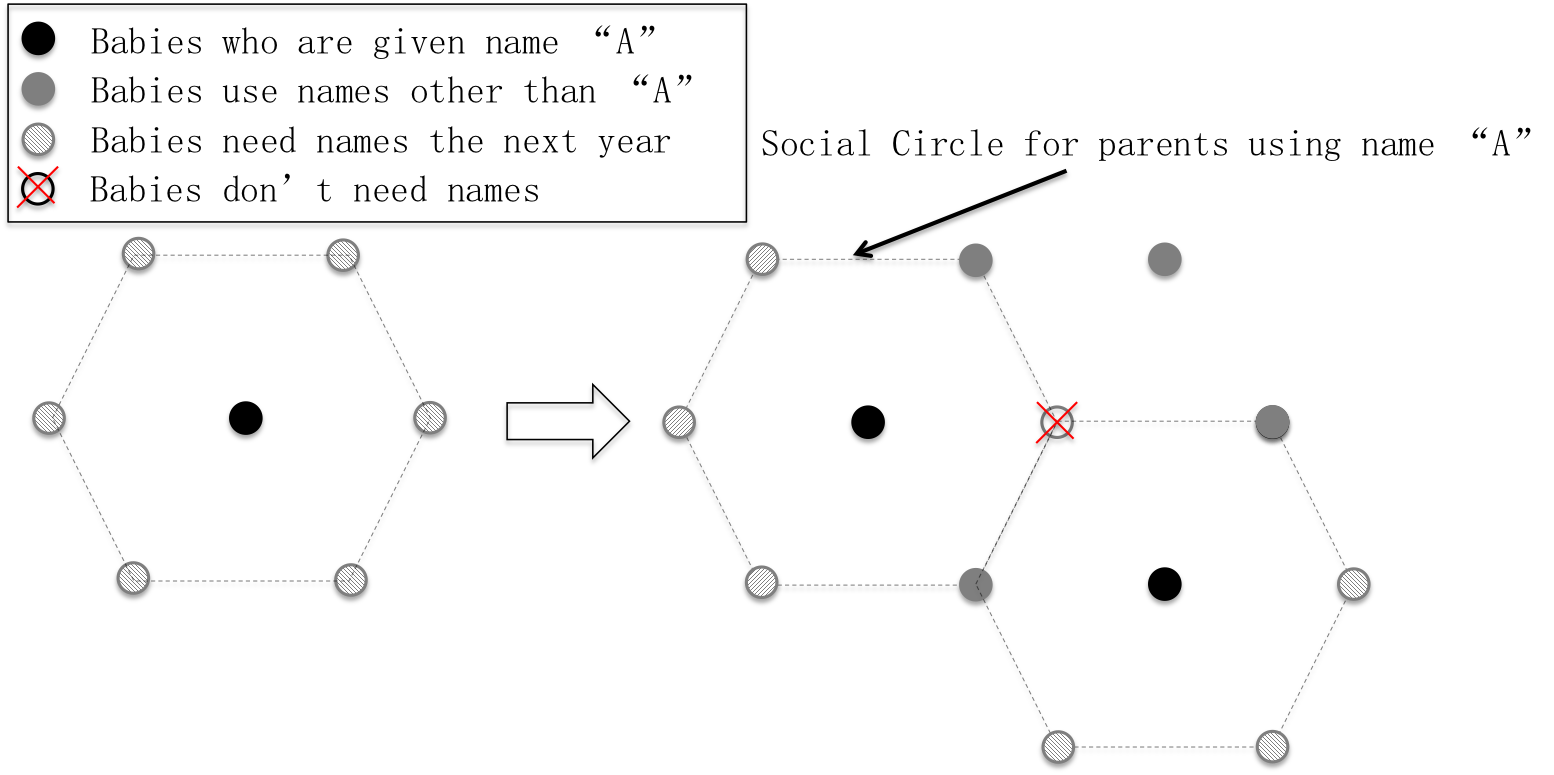
\includegraphics[width = 3.1in]{figure/EpidemicModelDiagram.png}
	\caption{Epidemic Model for Name}
	\label{fig:Epidemic Model for name}
\end{figure}

When one couple of parents first come up with a very lovely name, denote as name $i$ for their baby, they may not conceal this information to themselves, but to spread to everyone they may known. The baby who are lucky enough to get this name is like the black point in Fig. \ref{fig:Epidemic Model for name}. When friends, relatives and colleagues of the parents know this name, they may have a certain probability $p_i$ to give name $i$ to their babies. Those babies who need name for the next year are marked as hatched line points. When their babies use name $i$, new round of spreading starts. Of course, the probability of not using name $i$ is $1 - p_i$. In often the case, $p_i$ is small. So many babies may have gotten name rather than $i$. Gray points stand for babies use other names. Needless to say, the value of $p_i$ largely depends on how lovely name $i$ can be. But as a result of this step, $p_i$ for different names are not randomly scattered. Clearly, this model can only explain how one name becomes popular year after year. But this is enough for the prediction part for new names.

Now try to use mathematic language to describe this model more precisely.

At year $t$, the number of babies trying name $i$ is $y_{i, t}$. For the next year, babies given the same name is $y_{i, t + 1}$. If the probability of using name $i$ for one baby is $p_{i, t}$ and the total number of newborn babies in year $t + 1$ is $C_{t + 1}$, then we have:
\begin{align}
		& \frac{\partial y_{i, t + 1}}{\partial y_{i}} = p_{i, t} C_{t + 1}\\
	\Rightarrow &
		y_{i, t + 1} = p_{i, t} C_{t + 1} y_{i}\\
	\Rightarrow & 
		y_{i, t + 1} = y_{1}\prod_{k = 1}^t p_{k} C_{k + 1} \label{eq:number of babies given name i in year t+1 from year 1}
\end{align}

In Eq.\ref{eq:number of babies given name i in year t+1 from year 1}, $C_{t}$ can be calculated by compute the sum of all the occurrences of all names in year $t$, $y_{i, t}$ is the usage on name $i$ in year $t$, can also be got from the dataset. The only task remains is the estimation of $p_{i, t + 1}$. To simplify the model, and also based on the experimental result, we can use $\bar p_{i} = \frac{1}{t}\sum_{k = 1}^t p_{k}$ to approximate $\{p_{i, k}\}_{k = 1}^t$.
So 
\begin{align}
	p_{i, t} = \frac{y_{i, t + 1}}{y_{i} \cdot C_{t + 1}} \\
	p_i = \frac{1}{t}\sum_{k = 1}^t p_{k}
\end{align}

% subsection Epidemic Model for Name (end)

\subsection{Spreading Model for New Names} % (fold)
\label{sub:spreading_model_for_new_names}
Based on the assumptions and EMN model, we can build Spreading Model to predict trends for new names.

Similar to the model expressed in subsection \ref{sub:Epidemic Model for Name}, suppose in year $t$, a new name comes up with population $y_{t}$, then for year $t' (t' > t)$, we will have
\begin{align}
	y_{t'} = y_{t} \cdot \prod_{k = t + 1}^{t'} C_k \cdot \hat{p}
\end{align}

The $\hat{p}$ is the most likely $p$ among the estimation result for the previous subsection \ref{sub:Epidemic Model for Name}. 
\begin{align}
		\hat{p} = \max_p p\{ |\{p_i = p\}|, p_i \in P\} \label{ep:p_hat} \Leftrightarrow \hat{p} = MAP(p_i)
\end{align}

Note that, $P$ is the set for all the estimated $p_i$, and $|\cdot|$ is the operator to get the number of elements in a set.

% subsection spreading_model_for_new_names (end)
% section problem_formulation_&_models (end)

\section{Method} % (fold)
\label{sec:method}
Since the size of data is too large, there are 5647426 records in all, MySQL\cite{mysql2001mysql} database is implemented to store the data. The processing strategy is like below:
\begin{figure}[ht]
	\centering
	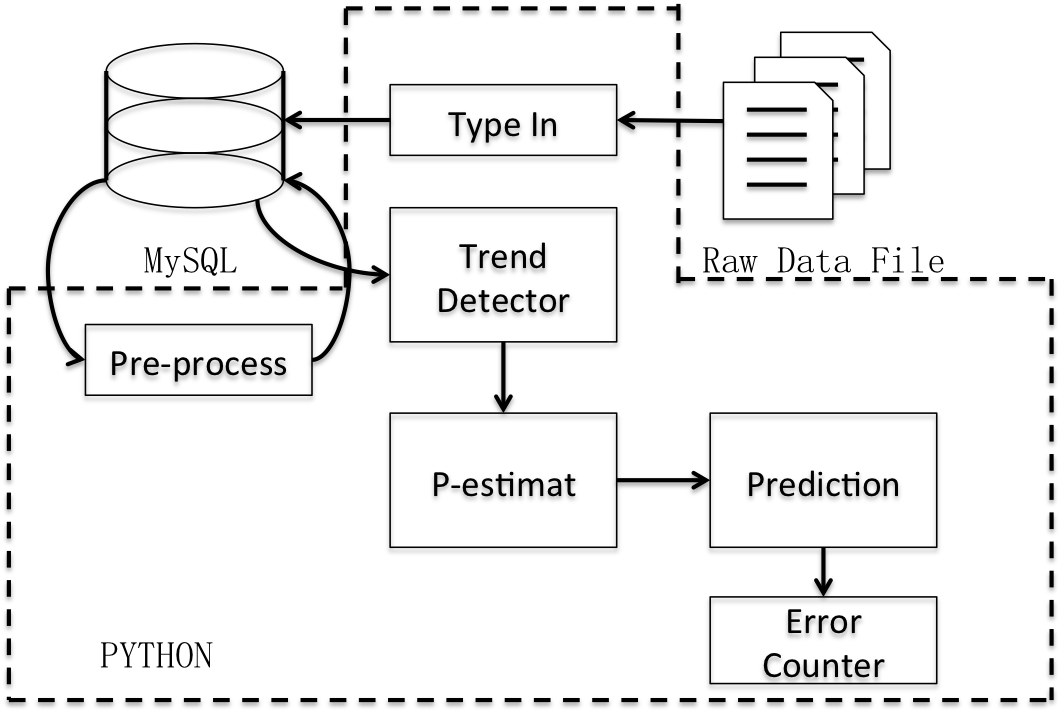
\includegraphics[width = 3.1in]{figure/implementation.png}
	\caption{Implementation Diagram}
	\label{fig:Implementation Diagram}
\end{figure}
\begin{enumerate}
	\item Type in: applying python script to type the datafile to the database;
	\item Pre-process: Combine data from different states, and sort names by their occurrence;
	\item Trend Detection: Apply the Matched-Filter based trend detector to get the incline part of the curve for each name;
	\item P-estimation: Use the Epidemic Model for Name to estimate $p$ for each name based on its incline period data;
	\item Prediction and Counting Error: Treat the last several years (from 1 to 5) as unknown, and calculate the prediction error for the model.
\end{enumerate}

% section method (end)


\section{Results} % (fold)
\label{sec:results}
The predicted figure for $p_{i, t}$ is like 
\begin{figure}[ht]
\centering
\subfigure[James]{
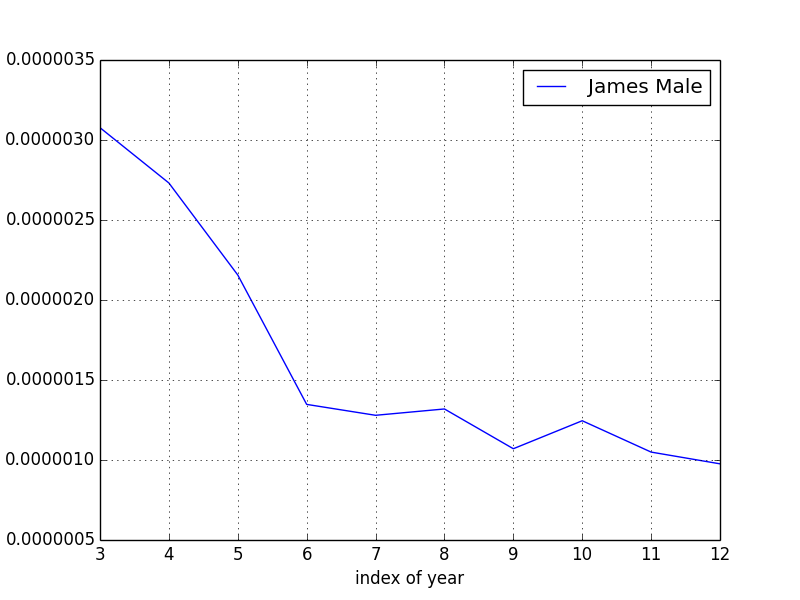
\includegraphics[width = 1.55in]{figure/p_est_for_James_male.png}
\label{fig:p_est for James}
}
\quad
\subfigure[Richard]{
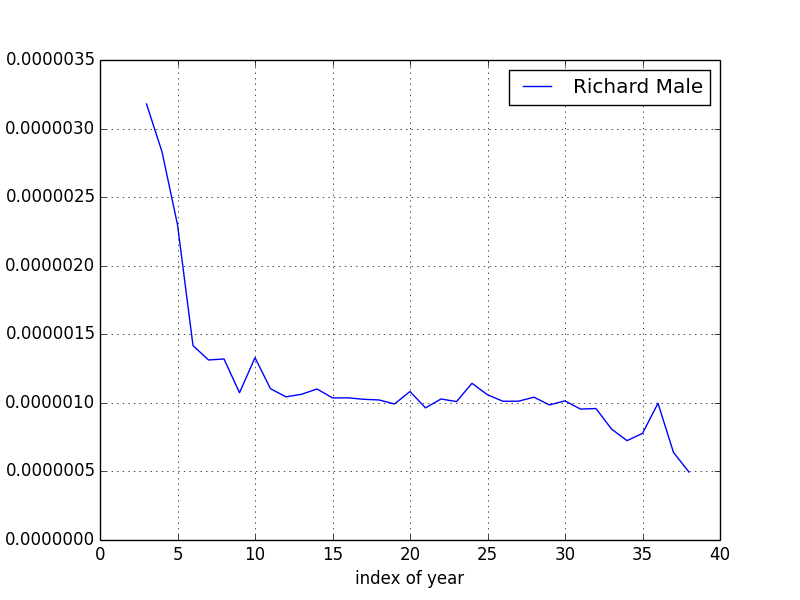
\includegraphics[width = 1.55in]{figure/p_est_for_Richard_male.png}
\label{fig:p_est for Richard}
}

\subfigure[Mary]{
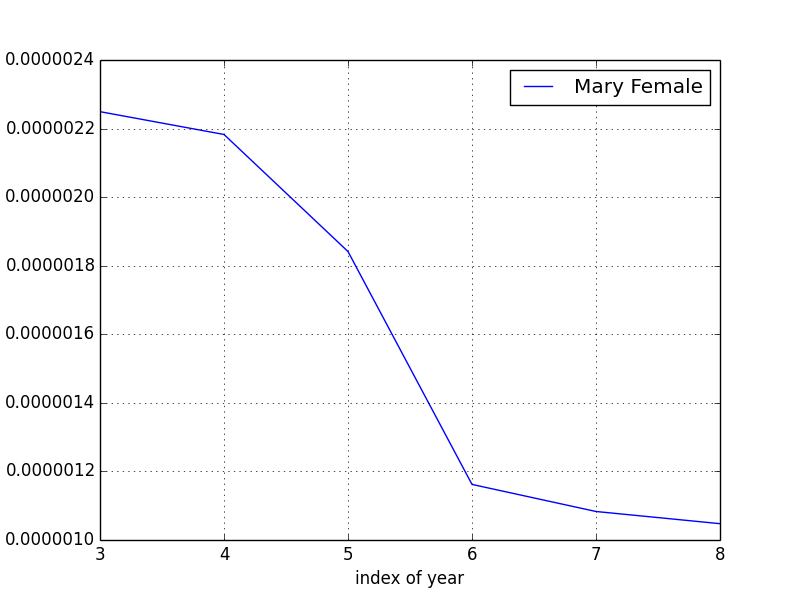
\includegraphics[width = 1.55in]{figure/p_est_for_Mary_female.png}
\label{fig:p_est for Mary}
}
\subfigure[Jennifer]{
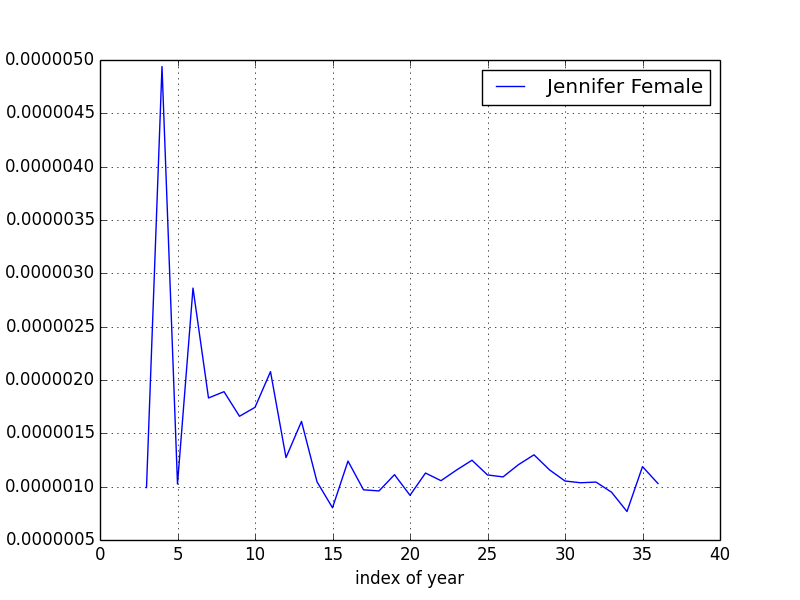
\includegraphics[width = 1.55in]{figure/p_est_for_Jennifer_female.png}
\label{fig:p_est for Jennifer}
}
\caption{Estimated P for Different Names}
\label{Estimated P for Different Names}
\end{figure}

The $p_{i, t}$ is not scattered randomly, but has a relatively stable value. So, using mean to represent the sequence of $\{p_{i, t}\}_{t = 1}^{t'}$ is reasonable.

Based on the model produced in section \ref{sub:Epidemic Model for Name}, the prediction error for female names is like Fig.\ref{fig:Prediction Error for Female Names}
\begin{figure}[ht]
	\centering
	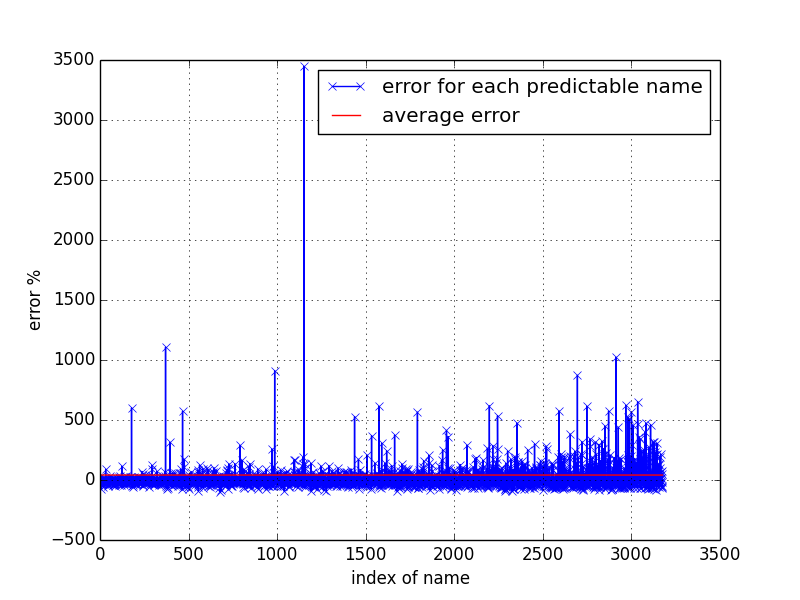
\includegraphics[width = 3.1in]{figure/error_female_13_9_1.png}
	\caption{Prediction Error for Female Names}
	\label{fig:Prediction Error for Female Names}
\end{figure}

The patten length is set to be $9$, and only predict one year. From the figure, except we know that some names have very large errors, most predictions have error within $5\%$.

The estimated error versus number of year to predict is like Fig. \ref{fig:Estimated Error vs Number of Year to Predict}.
\begin{figure}[ht]
	\centering
	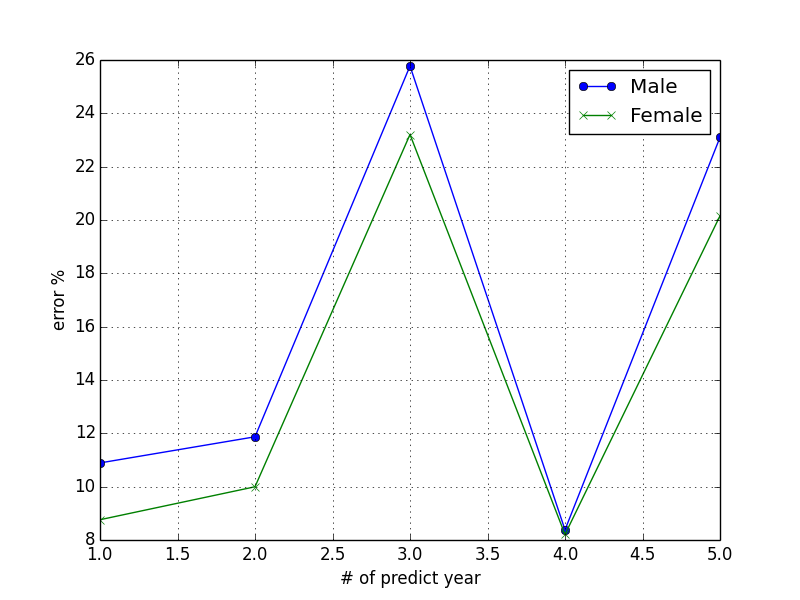
\includegraphics[width = 3.1in]{figure/error_vs_predictYear.png}
	\caption{Estimated Error vs Number of Year to Predict}
	\label{fig:Estimated Error vs Number of Year to Predict}
\end{figure}

So, the prediction for one or two years is more accurate than longer. But why the error for prediction of four years is the lowest is unknown. It may be the result of the law for the increasing trend of names.

\begin{figure}[ht]
	\centering
	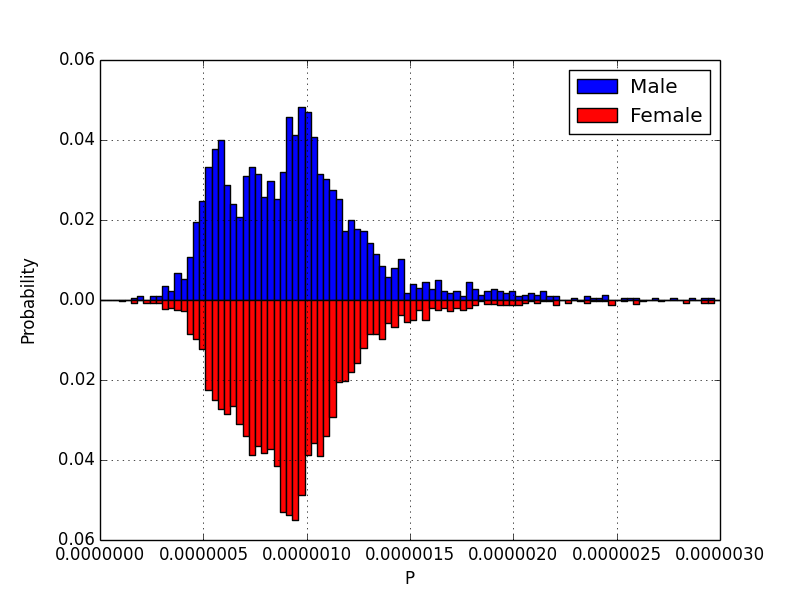
\includegraphics[width = 3.1in]{figure/pdf_for_p.png}
	\caption{pdf for Estimated P}
	\label{fig:pdf for Estimated P}
\end{figure}

Fig. \ref{fig:pdf for Estimated P} is the pdf for the estimated p. According to eq. \ref{ep:p_hat}, $p$ for female names and male names are in Table. \ref{Table:P for Prediction Model of New Names}.
\begin{table}[ht]
\centering
\begin{tabular}{c c c}
 \toprule
 &  male  & female\\ 
 \midrule
 p&  $9.6 \times 10^{-7}$  & $9.3 \times 10^{-7}$\\
 \bottomrule
\end{tabular}
\caption{P for Prediction Model of New Names}
\label{Table:P for Prediction Model of New Names}
\end{table}
% section results (end)
% section methodology (end)
\bibliographystyle{plain}
\bibliography{bibliography.bib}

% \begin{thebibliography}{1}
% \bibitem{SIS epidemic models}
% Allen L J S. Some discrete-time SI, SIR, and SIS epidemic models[J]. Mathematical biosciences, 1994, 124(1): 83-105.
% 
% \end{thebibliography}


\end{document}


